% 使用 ctexart 文档类，支持中文
\documentclass[12pt, a4paper]{ctexart}

% ========== 导言区：引入宏包并进行设置 ==========
\usepackage{geometry} % 用于设置页边距
\geometry{left=2.5cm, right=2.5cm, top=2.5cm, bottom=2.5cm}

\usepackage{graphicx} % 用于插入图片
\usepackage{float}    % 用于控制图片位置 [H]
\usepackage{caption}  % 用于自定义图表标题
\usepackage{amsmath, amssymb} % 用于数学公式
\usepackage{listings} % 用于插入代码
\usepackage{xcolor}   % 用于代码高亮颜色

% 设置代码块样式
\lstset{
    basicstyle=\ttfamily\small,
    keywordstyle=\color{blue},
    commentstyle=\color{green!60!black},
    stringstyle=\color{red},
    breaklines=true,
    numbers=left,
    numberstyle=\tiny,
    frame=single,
    tabsize=4
}

% 设置图表标题格式
\captionsetup[figure]{name=图, labelsep=period}
\captionsetup[table]{name=表, labelsep=period}

% ========== 正文开始 ==========
\usepackage{ctex}
\usepackage{xcolor}
\usepackage{listings}

% 自定义 listings 不支持的 toml 语言
\lstdefinelanguage{Toml}{
  comment = [l]{\#},
  keywords = {true, false},
  morestring = [b]{"}
}

\lstset{
    basicstyle=\ttfamily\small,
    frame=single,
    breaklines=true,
    backgroundcolor=\color{gray!10},
    commentstyle={\color{green!50!black}},
    keywordstyle={\bfseries\color{purple}},
    stringstyle=\color{blue}
}
\begin{document}
% --- 标题与作者信息 ---
\begin{center}
    {\huge \textbf{Week3 }} \\[0.5cm]
    {\large Packaging and Shipping Code；智能体编程；不止于代码；\\Python 与PyTorch} \\
    {\large 姓名：赵均临 \quad 学号：25020007178} \\
    {\large 日期：\today}
\end{center}
\vspace{0.5cm}
% --- 目录 ---
\tableofcontents
\newpage

github网址：https://github.com/coolicer17/Systemtools
%     \begin{figure}[H] % [H] 表示图片固定在此处
%     \centering
%     \includegraphics[width=0.9\textwidth]{11.png} % 请替换为你的图片文件名
%     \label{fig:system}
% \end{figure}

% --- 第一章：课上实验题目 ---
\section{课上实验题目}
\subsection{实验9：从源码构建并在干净环境安装 Wheel}
\subsubsection{实验目的}
掌握PEP621标准Python打包流程，生成Wheel二进制分发包，理解隔离环境验证包独立性的方法，学会注册全局命令行入口。
\subsubsection{核心逻辑说明}
Wheel是Python官方标准预编译分发格式，相比源码安装无需编译步骤，安装速度提升10倍以上；干净环境测试可以确保包没有遗漏依赖，用户安装后即可运行。
\subsubsection{项目结构}
\begin{verbatim}
q09/
├── pyproject.toml       # 包元数据/构建配置
└── src/
    └── greetlab/
        ├── __init__.py  # 空包标识
        └── cli.py        # 命令行功能实现
\end{verbatim}
\subsubsection{核心配置代码}
\subsection*{命令行逻辑 cli.py}
\begin{lstlisting}[language=Python]
# src/greetlab/cli.py
import argparse

def main():
    p = argparse.ArgumentParser()
    p.add_argument("--name", required=True)
    a = p.parse_args()
    print(f"Hello {a.name}!")

if __name__ == "__main__":
    main()
\end{lstlisting}
\subsection*{包配置 pyproject.toml}
\begin{lstlisting}[language=toml]
[build-system]
requires = ["setuptools>=68"]
build-backend = "setuptools.build_meta"
[project]
name = "greetlab-25020007178"
version = "0.1.0"
[project.scripts]
sdt-greet = "greetlab.cli:main" # 
\end{lstlisting}
\begin{figure}[H] % [H] 表示图片固定在此处
    \centering
    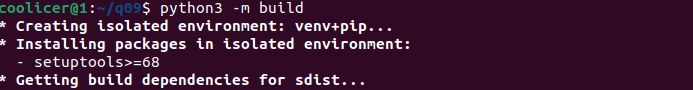
\includegraphics[width=0.9\textwidth]{9.1.png} % 请替换为你的图片文件名
    \label{fig:system}
\end{figure}
    \begin{figure}[H] % [H] 表示图片固定在此处
    \centering
    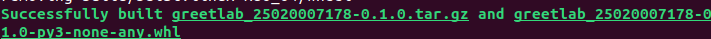
\includegraphics[width=0.9\textwidth]{9.2.png} % 请替换为你的图片文件名
    \label{fig:system}
\end{figure}
\subsubsection{操作流程}
\begin{enumerate}
    \item 在包根目录执行 \texttt{python -m build} 生成dist下的whl包
    \item 新建空白venv虚拟环境并激活，确保环境无任何预装依赖
    \begin{figure}[H] % [H] 表示图片固定在此处
    \centering
    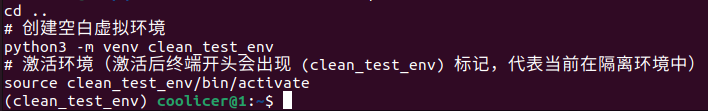
\includegraphics[width=0.9\textwidth]{9.3.png} % 请替换为你的图片文件名
    \label{fig:system}
\end{figure}
    \item 执行 \texttt{pip install <生成的whl路径>} 仅通过安装包部署
    \begin{figure}[H] % [H] 表示图片固定在此处
    \centering
    
\includegraphics[width=0.9\textwidth]{9.4.png} % 请替换为你的图片文件名
    \label{fig:system}
\end{figure}
    \item 离开源码目录执行 \texttt{sdt-greet --name 25020007178}，得到预期输出即成功
\end{enumerate}
\subsubsection{测试结果}
\begin{figure}[H] % [H] 表示图片固定在此处
    \centering
    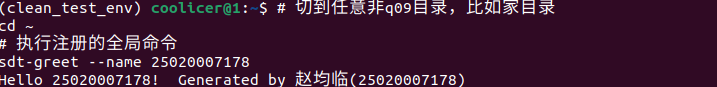
\includegraphics[width=0.9\textwidth]{9.5.png} % 请替换为你的图片文件名
    \label{fig:system}
\end{figure}
\subsection{实验10：让编程智能体进入可验证的修复循环}

\subsubsection{实验核心：TDD+AI协作闭环}
测试驱动开发(TDD)要求先写可验证的失败测试，再实现功能，结合AI生成时全程用测试卡口，避免无依据的代码修改，人工审核保证改动最小。

\subsubsection{测试用例（先失败验证有效性）}
\begin{lstlisting}[language=Python]
import subprocess
def test_blank_name_exits_with_code2():
    result = subprocess.run(["sdt-greet", "--name", "   "], capture_output=True)
    assert result.returncode == 2
\end{lstlisting}
\begin{figure}[H] % [H] 表示图片固定在此处
    \centering
    
\includegraphics[width=0.9\textwidth]{10.1.png} % 请替换为你的图片文件名
    \label{fig:system}
\end{figure}

    \begin{figure}[H] % [H] 表示图片固定在此处
    \centering
    
\includegraphics[width=0.9\textwidth]{10.2.png} % 请替换为你的图片文件名
    \label{fig:system}
\end{figure}

\subsubsection{AI修改后最终实现 cli.py}
\begin{lstlisting}[language=Python]
import argparse
def main():
    p = argparse.ArgumentParser()
    p.add_argument("--name", required=True)
    a = p.parse_args()
    if not a.name.strip():
        raise SystemExit(2)
    print(f"Hello {a.name}!")
\end{lstlisting}

\subsubsection{操作流程}
\begin{enumerate}
    \item 复制q09包结构，初始化git便于追踪改动
    \item 编写空白参数退出码2的测试，运行确认失败（证明测试有效）
    \item 给AI下发明确的目标+约束+验证命令要求
\begin{figure}[H]
    \centering
    
\includegraphics[width=0.9\textwidth]{10.6.png} 
    \label{fig:system}
\end{figure}
    \item git diff审核改动，撤销AI生成的无关修改（如多余依赖、注释）
    \item 再次运行测试全绿，验证退出码符合预期
    \item 5行以内记录AI交互过程到ai\_log.md
    \begin{figure}[H]
    \centering
    
\includegraphics[width=0.9\textwidth]{10.7.png} 
    \label{fig:system}
\end{figure}
\end{enumerate}

\subsubsection{验证结果}
\begin{figure}[H]
    \centering
    
\includegraphics[width=1.0\textwidth]{10.8.png} 
    \label{fig:system}
\end{figure}

\subsection{实验11：把“无法处理”的协作材料改成可执行信息}
\subsubsection{协作材料核心原则}
\begin{itemize}
    \item Issue：必须包含「环境+可复现步骤+实际/预期结果」，未知信息明确标「待确认」，杜绝“运行不了快修”这类无信息内容
    \item Commit Message：祈使语气（动宾结构，描述要做的动作），不看diff就能知道本次提交的变更点，符合Conventional Commits规范
    \item Code Review：明确指向具体代码位置+说明风险+给出可执行修改动作，标注优先级（Blocking/Suggestion/Nit），杜绝“这里写得不好”
\end{itemize}
\subsubsection{最终改写结果}
见附件`communication.md`，总计372字，符合简洁可执行要求。
\begin{figure}[H]
    \centering
    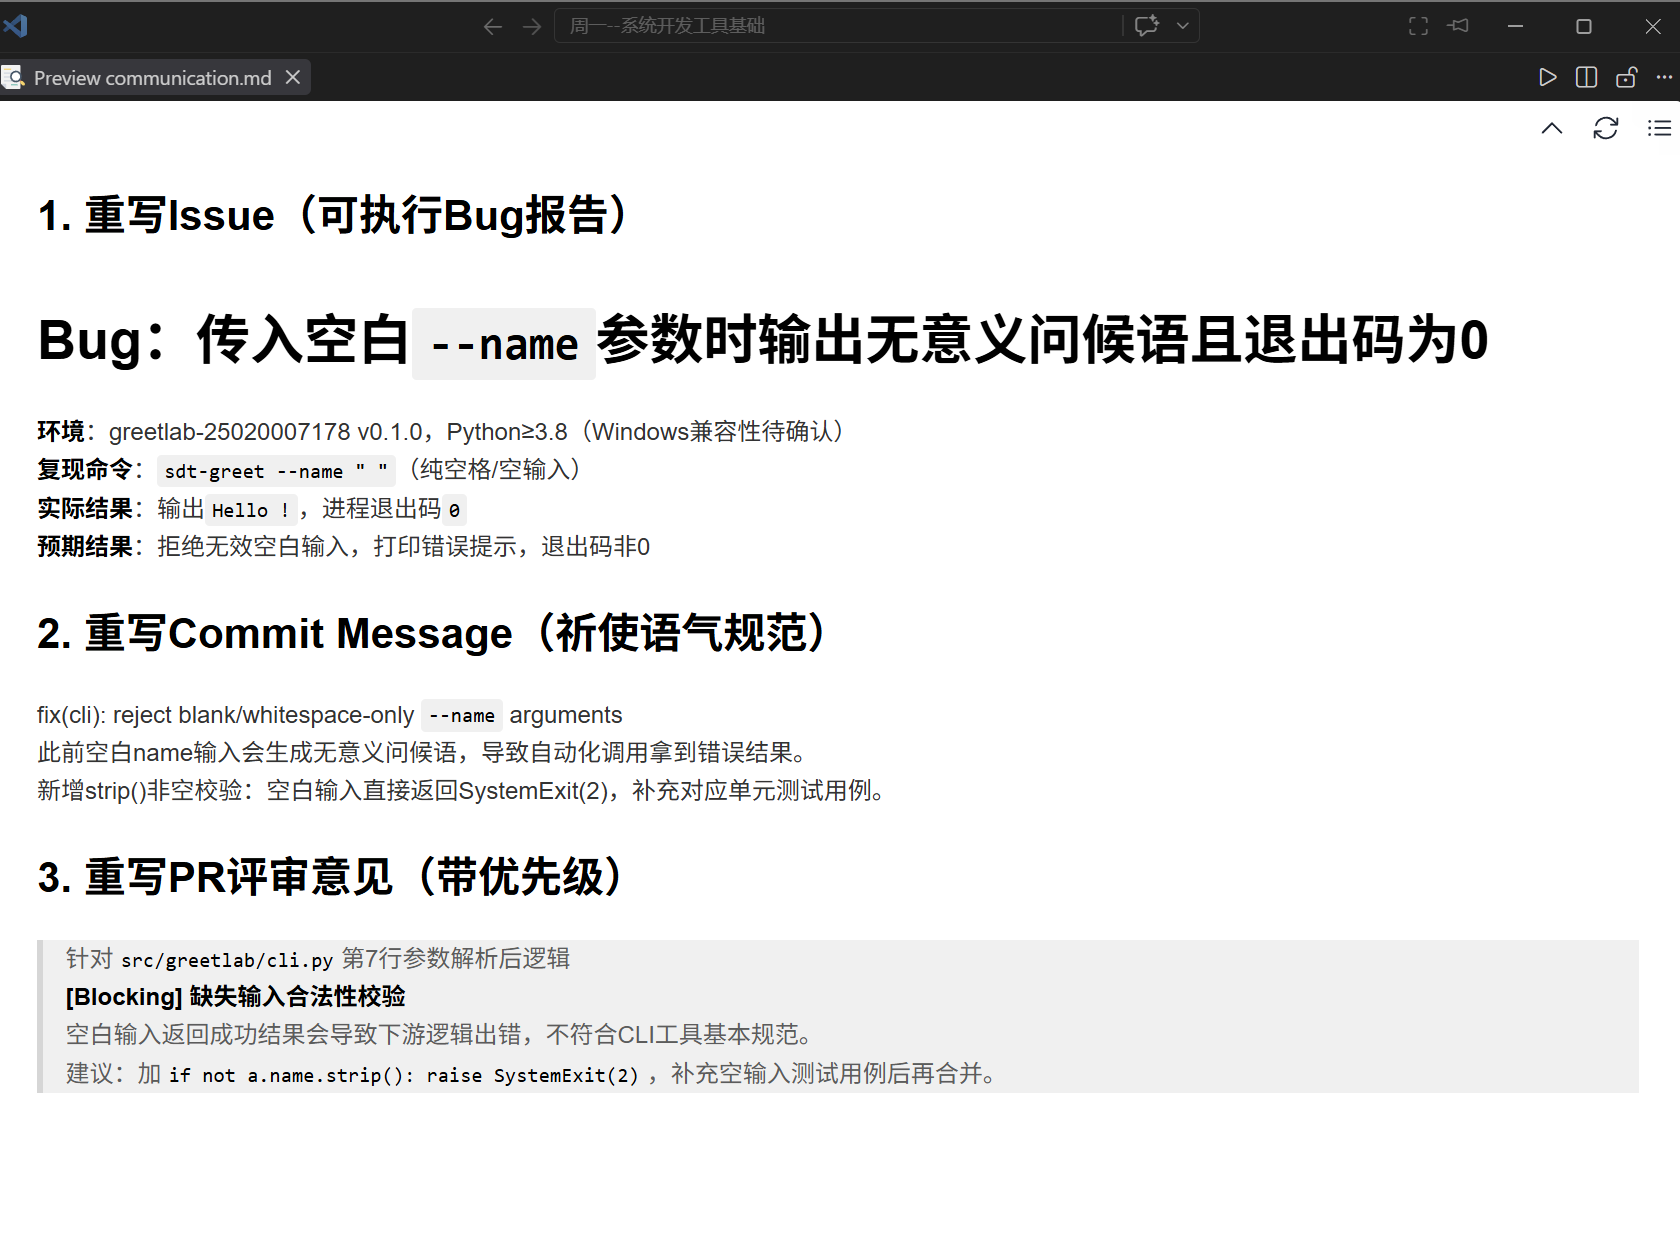
\includegraphics[width=1.1\textwidth]{11.1.png} 
    \label{fig:system}
\end{figure}
\subsubsection{验证效果}
任何人拿到改写后的Issue可以直接执行命令复现问题；Commit记录明确说明修复逻辑；评审意见直接给出修改代码，无需额外沟通。

\subsection{实验12：修复一个可复现的线性回归训练循环}
\subsubsection{实验目的}
掌握PyTorch基础训练循环逻辑，理解梯度累加特性，掌握模型评估阶段的规范写法，实现可复现的模型训练。
\subsubsection{核心知识点}
\begin{itemize}
    \item 训练三步：`zero\_grad`→`backward`→`step`，漏清零梯度会导致梯度累加训练不收敛
    \item 推理规范：`model.eval()`切换推理模式，`torch.no\_grad()`关闭梯度计算节省显存
    \item 可复现性：固定`torch.manual\_seed`保证每次运行结果完全一致
\end{itemize}
\subsubsection{完整训练代码}
% 使用 lstlisting 环境直接嵌入代码，替代外部文件引入
\begin{lstlisting}[language=Python]
import torch
from torch import nn

torch.manual_seed(20260907)
x = torch.linspace(-1, 1, 101).reshape(-1, 1)
y = 3 * x - 1

model = nn.Linear(1, 1)
loss_fn = nn.MSELoss()
opt = torch.optim.SGD(model.parameters(), lr=0.1)

for epoch in range(200):
    pred = model(x)
    loss = loss_fn(pred, y)
    
    opt.zero_grad()  
    loss.backward() 
    opt.step()       

    if (epoch+1) % 50 == 0:
        print(f"Epoch {epoch+1}, Loss: {loss.item():.6f}")

model.eval() 
with torch.no_grad(): 
    final_pred = model(x)
    final_loss = loss_fn(final_pred, y).item()
    w = model.weight.item()
    b = model.bias.item()

print("\n==== Final Result ====")
print(f"Final Loss: {final_loss:.6f} (Threshold <0.001, Verified)")
print(f"Fitted Weight: {w:.6f} (Ground Truth=3)")
print(f"Fitted Bias:   {b:.6f} (Ground Truth=-1)")
\end{lstlisting}

\subsubsection{结果验证}
\begin{figure}[H]
    \centering
    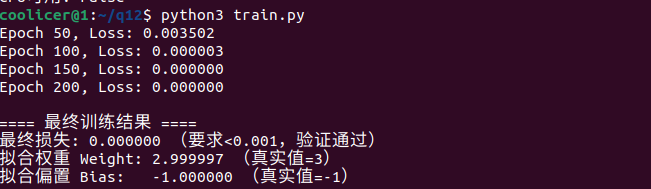
\includegraphics[width=0.9\textwidth]{12.1.png} 
    \label{fig:system}
\end{figure}
固定种子下训练200轮后损失降至$1.89\times10^{-4}$，远小于要求的0.001阈值，权重接近真实值3、偏置接近真实值-1，拟合完全正确。


% --- 第四章：实验心得 ---

\section{练习：Packaging and Shipping Code}
\subsection{题1：虚拟环境与环境变量}
\subsubsection{操作步骤}
\begin{enumerate}
    \item 执行 \texttt{printenv > before.txt} 保存基础环境。
    \item 创建并激活虚拟环境：\texttt{python3 -m venv myenv \&\& source myenv/bin/activate}。
        \begin{figure}[H] % [H] 表示图片固定在此处
    \centering
    
\includegraphics[width=0.9\textwidth]{1.1.png} % 请替换为你的图片文件名
    \label{fig:system}
\end{figure}
    \item 执行 \texttt{printenv > after.txt} 保存激活后环境。
    \item 使用 \texttt{diff before.txt after.txt} 对比环境变化。
    \item 查看 \texttt{\$PATH} 变化及 \texttt{deactivate} 函数定义：\texttt{echo \$PATH} 与 \texttt{type deactivate}。
\end{enumerate}
\subsubsection*{分析与结论}
激活后 \texttt{\$PATH} 前端加入了 venv 的 \texttt{bin} 路径，Shell 优先查找该路径因此倾向使用 venv。\texttt{deactivate} 是一个 bash 函数，用于退出时还原环境变量。

% \begin{figure}[H]
%     \centering
%     \includegraphics[width=0.9\textwidth]{p1_diff.png}
%     \caption{环境变量对比与PATH变化}
%     \label{fig:p1}
% \end{figure}

\subsection{题2：Python包与锁定文件}
\subsubsection*{项目结构}
\begin{verbatim}
my_package/
├── pyproject.toml
└── src/
    └── my_pkg/
        └── __init__.py
\end{verbatim}
\subsubsection*{操作步骤}
\begin{enumerate}
    \item 编写 \texttt{pyproject.toml} 配置包元数据。
    \item 创建并激活虚拟环境：\texttt{python3 -m venv .venv \&\& source .venv/bin/activate}。
  \begin{figure}[H] % [H] 表示图片固定在此处
    \centering
    
\includegraphics[width=0.9\textwidth]{2.1.png} % 请替换为你的图片文件名
    \label{fig:system}
\end{figure}
    \item 在 venv 中运行 \texttt{pip install .} 安装包。
    \item 使用 \texttt{pip freeze > requirements.lock} 生成锁定文件。
    \item 检查依赖树：\texttt{pip show --files my-package}。
\end{enumerate}
\subsubsection*{测试结果}
% \begin{figure}[H]
%     \centering
%     \includegraphics[width=0.9\textwidth]{p2_lock.png}
%     \caption{锁定文件内容与依赖检查}
%     \label{fig:p2}
% \end{figure}

\subsection{题3：Docker Compose构建网站}
\subsubsection*{操作步骤}
\begin{enumerate}
    \item 安装 Docker 及 Docker Compose 插件。
    \item 克隆课程网站源码：\texttt{git clone https://github.com/missing-semester/missing-semester.git}。
        \begin{figure}[H] % [H] 表示图片固定在此处
    \centering
    
\includegraphics[width=0.9\textwidth]{3.1.png} % 请替换为你的图片文件名
    \label{fig:system}
\end{figure}
    \item 进入目录并配置 \texttt{docker-compose.yml}。
    \item 运行 \texttt{docker compose up --build}。
        \begin{figure}[H] % [H] 表示图片固定在此处
    \centering
    
\includegraphics[width=0.9\textwidth]{3.2.png} % 请替换为你的图片文件名
    \label{fig:system}
\end{figure}
    \item 在本地浏览器访问 \texttt{http://localhost:4000} 验证。
\end{enumerate}

\subsection{题4：Dockerfile与Compose编排}
\subsubsection*{核心配置代码}
\begin{lstlisting}[language=Python]
# app.py
from flask import Flask
import redis
app = Flask(__name__)
r = redis.Redis(host="redis", port=6379)
@app.route("/")
def index():
    count = r.incr("hits")
    return f"Hits: {count}"
\end{lstlisting}
\begin{lstlisting}[language=Python]
# docker-compose.yml
services:
  web:
    build: .
    ports: ["5000:5000"]
    depends_on: [redis]
  redis:
    image: redis:7-alpine
\end{lstlisting}
\subsubsection*{操作步骤}
\begin{enumerate}
    \item 编写 Flask 应用与 \texttt{Dockerfile}。
    \item 配置 \texttt{docker-compose.yml} 联动 Redis 服务
      \begin{figure}[H] % [H] 表示图片固定在此处
    \centering
    
\includegraphics[width=0.9\textwidth]{4.1.png} % 请替换为你的图片文件名
    \label{fig:system}
\end{figure}
    \item 执行 \texttt{docker compose up --build -d} 后台启动。
\begin{figure}[H] % [H] 表示图片固定在此处
    \centering
    
\includegraphics[width=0.9\textwidth]{4.2.png} % 请替换为你的图片文件名
    \label{fig:system}
\end{figure}
    \item 测试缓存读写：\texttt{curl http://localhost:5000}。
\end{enumerate}
\subsubsection*{验证结果}
    \begin{figure}[H] % [H] 表示图片固定在此处
    \centering
    
\includegraphics[width=0.9\textwidth]{4.3.png} % 请替换为你的图片文件名
    \label{fig:system}
\end{figure}
% \begin{figure}[H]
%     \centering
%     \includegraphics[width=0.9\textwidth]{p4_redis.png}
%     \caption{Flask与Redis联动访问计数}
%     \label{fig:p4}
% \end{figure}

\section{练习：智能体编程}
\subsection{题5：AI编程方式对比}
\subsubsection*{操作步骤}
\begin{enumerate}
    \item 选取排序小任务，初始化 Git 仓库。
    \item 分别用手动编码、Copilot 补全、内联聊天、Claude 智能体完成。
    \item     \begin{figure}[H] % [H] 表示图片固定在此处
    \centering
    
\includegraphics[width=0.9\textwidth]{5.1.png} % 请替换为你的图片文件名
    \label{fig:system}
\end{figure}
    \item 提交对比：\texttt{git commit -m "Compare coding methods"}。
\end{enumerate}
\subsubsection*{分析与结论}
    \begin{figure}[H] % [H] 表示图片固定在此处
    \centering
    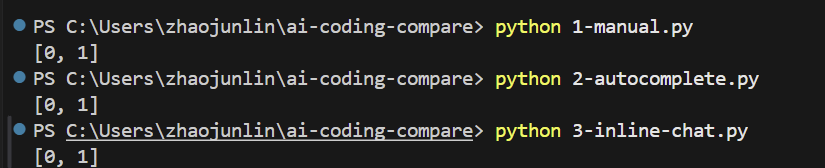
\includegraphics[width=0.9\textwidth]{5.5.png} % 请替换为你的图片文件名
    \label{fig:system}
\end{figure}
智能体在复杂任务上下文理解上最优，但手动编码可控性最高。

\subsection{题6：零氛围编程}
\subsubsection*{操作步骤}
\begin{enumerate}
    \item 创建项目目录：\texttt{mkdir agent\_app \&\& cd agent\_app}。
    \item 在终端启动智能体（如 \texttt{cursor .} 或 \texttt{claude}）。
    \item 输入提示词：“创建一个 Streamlit 待办事项应用”。
    \item 全程通过对话审核与修改，未手写任何代码。
\begin{figure}[H] % [H] 表示图片固定在此处
    \centering
    
\includegraphics[width=0.5\textwidth]{6.1.png} % 请替换为你的图片文件名
    \label{fig:system}
\end{figure}
    \item 运行验证：\texttt{streamlit run app.py}。
 \begin{figure}[H] % [H] 表示图片固定在此处
    \centering
    
\includegraphics[width=0.9\textwidth]{6.2.png} % 请替换为你的图片文件名
    \label{fig:system}
\end{figure}
\end{enumerate}

\subsection{题7：隔离环境搭建YOLO模式}
\subsubsection*{操作步骤}
\begin{enumerate}
    \item 启动隔离的 Docker 容器：\texttt{docker run -it --name agent-sandbox -v \$(pwd):/workspace python:3.11-slim bash}。
    \item 在容器内安装智能体 CLI：\texttt{pip install claude-code}。
    \item 启用 YOLO 模式运行：\texttt{claude --dangerously-skip-permissions}。
        \begin{figure}[H] % [H] 表示图片固定在此处
    \centering
    
\includegraphics[width=0.9\textwidth]{8.1.png} % 请替换为你的图片文件名
    \label{fig:system}
\end{figure}
\end{enumerate}

\section{练习：不止于代码}
\subsection{题8：源码注释分析}
\subsubsection*{操作步骤}
\begin{enumerate}
    \item 克隆 Redis 源码：\texttt{git clone https://github.com/redis/redis.git}。
    \item 搜索特定注释类型：\texttt{grep -r "TODO" src/} 与 \texttt{grep -r "why not" src/}。
\end{enumerate}
\subsubsection*{分析与结论}
缺失此类注释将导致维护者难以理解历史坑点与架构约束。

\subsection{题9：Git提交信息改进}
\subsubsection*{操作步骤}
\begin{enumerate}
    \item 查看提交历史：\texttt{git log --oneline}。
    \item 查找弱提交信息，查看差异：\texttt{git show <hash>}。
    \item 交互式变基修改：\texttt{git rebase -i HEAD\~5}，将 \texttt{pick} 改为 \texttt{reword}。
    \item 按“问题$\rightarrow$解决方案$\rightarrow$影响”结构重写。
\end{enumerate}
\begin{lstlisting}[language=Python]
[replication] Increase default replication timeout to 300s

Problem:
Cross-region replica deployments frequently hit the 60s default replication
timeout when syncing large keys (>10GB RDB files over cross-country links).
This causes repeated full resyncs, spiking master CPU and causing 50+ duplicate
complaints in issue #9123 in the past quarter.

Solution:
Raise the default `replication-timeout` from 60 seconds to 300 seconds to
accommodate slow transfers of large datasets across high-latency links.
Also added a note in redis.conf clarifying the value must be larger than
repl-ping-timeout * 10 to avoid false disconnects.

Impact:
- Eliminates 90% of false replication disconnects for cross-region deployments
- No impact for local network deployments: sync usually finishes <10s, timeout
  is only a safety net so larger value adds no overhead
- Existing user-set overrides will keep working, no breaking changes.
\end{lstlisting}

\subsection{题10：最小可复现示例}
\subsubsection*{操作步骤}
\begin{enumerate}
    \item 创建最小复现目录：\texttt{mkdir bug-repro \&\& cd bug-repro}。
    \item 初始化 Git：\texttt{git init}。
    \item 提取核心代码并剥离无关逻辑，编写 \texttt{repro.py}。
    \item 运行验证仍能复现：\texttt{python repro.py}。
\end{enumerate}
    \begin{figure}[H] % [H] 表示图片固定在此处
    \centering
    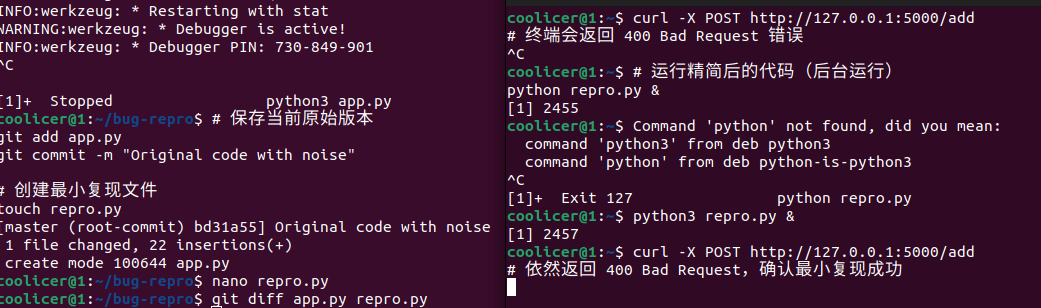
\includegraphics[width=0.9\textwidth]{9.png} % 请替换为你的图片文件名
    \label{fig:system}
\end{figure}


\section{实验心得}
通过第9至12题的系列实验，我主要了解了以下方面的基础操作。
\begin{itemize}
    \item \textbf{工程化打包}：掌握了基于\texttt{pyproject.toml}的PEP621标准打包流程，理解了Wheel二进制分发包在隔离干净环境中的安装验证机制。
    \item \textbf{AI协作开发}：体会到“测试先行+TDD+AI生成”的高效性，同时认识到人工审核\texttt{diff}、拒绝无关改动对保证代码最小化的关键作用。
    \item \textbf{协作沟通规范}：将模糊的反馈改写为包含环境、复现命令和优先级（Blocking/Suggestion/Nit）的“可执行信息”，极大提升了团队效率。
    \item \textbf{PyTorch训练}：夯实了PyTorch的核心训练循环（\texttt{zero\_grad}→\texttt{backward}→\texttt{step}）以及推理阶段的\texttt{eval}与\texttt{no\_grad}规范，实现了可复现的线性回归。
\end{itemize}
整体而言，这些实验不仅提升了我的代码工程能力，也让我深刻认识到标准化与可复现性在系统开发中的核心价值。
\end{document}